\documentclass[12pt]{article}
\DeclareMathSizes{12}{13}{10.4}{10.4}
\usepackage[utf8]{inputenc}
\usepackage[margin=1.5cm]{geometry}
\usepackage{amsmath}
\usepackage{amssymb}
\usepackage{cancel}
\usepackage{graphicx}

\begin{document}
\section*{LEZIONE 7: COSTO COMPUTAZIONALE DEGLI ALGORITMI NUMERICI}
Nelle scorse lezioni abbiamo familiarizzato con altri concetti cardine del calcolo numerico\\
\textbf{CONVERGENZA:}\\
la maggior parte dei metodi numerici prevede la costruzione di una successione 
di "oggetti" (numeri, vettori, funzioni) che convergono in senso opportuno ad un oggetto limite, che è l'oggetto da approssimare, si tratta di un processo infinito (passaggio al limite) che va "fermato", 
quando tramite opportune stime l'approssimazione è entrata in un prefissato intorno del limite, determinato da una "tolleranza".\\
Lo schema tipico è 
\begin{equation}
    ERRORE(n) \lesssim STIMA(n) \leq TOLL
\end{equation}
\begin{center}
    dove
\end{center}
\begin{center}
    $ERRORE(n) = e_n = |X_n-e|$
\end{center}
\begin{center}
    $TOLL = \epsilon$
\end{center}
dove si è dimostrato teoricamente che $x_n\rightarrow l$ cioè $e_n\rightarrow0$,$n\rightarrow\infty$
\\
\textbf{STABILITA':}\\
In tutti gli algoritmi numerici, anche quelli che fanno a priori un numero finito di passi, (come alcuni algoritmi dell'algebra lineare, ad es. il metodo di eliminazione di Gauss), vengono introdotti errori durante il processo di calcolo, a partire dagli inevitabili errori di arrotondamento, ad errori di misura dei dati, dovuti ad un algoritmo secondario che fornisce all'algoritmo primario dei risultati approssimati da elaborare (ad esempio un algoritmo che approssima uno zero di funzione che a sua volta viene approssimato tramite uno sviluppo di serie).\\
Come abbiamo già visto con vari esempi, cerchiamo di evitare algoritmi che propagano male gli errori amplificandoli, cioè cerchiamo algoritmi che oltre ad essere \textit{convergenti} siano anche \textit{stabili} (si pensi alla successione di Archimede per $\pi$ nella versione instabile che abbiamo poi stabilizzato).\\
Ma accanto a questi due concetti, ce n'è un terzo che ci dice quando un algoritmo di approssimazione è ben utilizzabile in pratica, ed è il concetto di\\
\textbf{EFFICIENZA:}\\
tra i vari algoritmi che risolvono un problema, siamo interessati a quelli che hanno un basso \textit{costo computazionale} (ovviamente a parità di errore, visto che in questo corso trattiamo algoritmi numerici cioè algoritmi che forniscono non un risultato esatto ma un risultato approssimato a meno di una certa tolleranza). Si pensi ad esempio, per fissare le idee, all'algoritmo di Archimede per il calcolo di $\pi$ che ha chiaramente parità di errore un costo molto più basso dell'algoritmo basato sulla serie armonica, visto che la convergenza è molto più rapida.\\\\
Ma come si misura il costo computazionale di un algoritmo numerico?\\ Consideriamo sostanzialmente  due parametri:
\begin{itemize}
    \item NUMERO DI FLOPS (floating-point operations)
    \item TEMPO DI CALCOLO 
\end{itemize}
Ovviamente il numero di operazioni floating-point influenza il tempo di calcolo attraverso la velocità del processore, che si misura in flops/sec, ad esempio un processore da 1 Gflops/sec (Gigaflops) fa $10^9$ flops al secondo, che è l'ordine di grandezza per il processore di un PC attuale (mentre i super-computer hanno ormai raggiunto i Pflops (Petaflops, $10^{15}$ flops/sec) e la tecnologia sta puntando all'Eflops (Exaflops, $10^{18}$ flops/sec).\\ Ma il tempo effettivo di calcolo, che è il parametro più importante dal punto di vista pratico (si pensi in particolare agli algoritmi "real-time" che devono fornire una risposta entro un tempo predefinito, in scale di tempi dipendenti dal problema, ad es. frazioni di secondo per il controllo numerico di un macchinario industriale oppure ore/giorni nella simulazione dei modelli estremamente complessi per le previsioni meteo).\\ In effetti il tempo di calcolo, oltre che dalla velocità del processore è influenzato anche dalla \underline{velocità dei flussi dati} tra le varie parti della memoria del computer, ed è un parametro che dipende dal tipo di computer ("machine dependent" come si dice in inglese informatico).\\
Invece il \#flops ha il vantaggio di essere "machine independent" e di dare quindi una misura parzialmente incompleta ma in un certo senso "universale" del costo computazionale di un dato algoritmo numerico. \\
Per capire l'effetto dei flussi di dati fra le diverse zone di memoria del computer in algoritmi che lavorano su grandi masse di dati, facciamo un esempio un po' ingenuo ma indicativo con un modello di computer molto semplificato, solo per fissare le idee. Come è noto, la velocità di scambio dati con la memoria centrale (accesso veloce) può essere maggiore di vari ordini di grandezza rispetto allo scambio dati con l'hard-disk o altre memoria di massa. \\ Conviene quindi implementare gli algoritmi che lavorano in masse di dati e hanno bisogno delle memorie ad accesso più lento, minimizzando i flussi dati. Prendiamo il seguente modello\\
\begin{equation*}
    PROCESSORE <----> MEM. CENTRALE    (RAM) <----> HARD-DISK
\end{equation*}
e supponiamo di dover fare il prodotto di due matrici $A,B\in \mathbb{R}^{n\cdot m}$, con il vincolo che nella memoria centrale si può memorizzare solo 1 matrice e qualche vettore di dimensione n, ma non due matrici.\\Chaimiamo come spesso si fa in letteratura "FLOAT" un reale-macchina.\\
La situazione descritta non è irrealistica: con una RAM di 8 GB possiamo memorizzare $\frac{8\cdot10^9}{8}=10^9$ floats, cioè 1 miliardo di floats a 64 bits= 8 bytes (1 Byte= 8bit).\\
Quindi se n=30000, ogni matrice occupa $n^2=9\cdot 10^8$ floats e nella RAM non ci stanno entrambe le matrici A e B, una delle due, ad es.B, deve essere memorizzata nell'hard disk, così come la matrice prodotto $C=AB$.\\
Ricordiamo che 
\begin{equation*}
    c_{ij}=\sum_{k=1}^n a_{ik}b_{kj}
\end{equation*}
cioè $c_{ij}$ è il prodotto della \underline{riga i} di A con la \underline{colonna j} di B, $R_{i}(A)\cdot C_{j}(B)$\\
È chiaro che il costo del calcolo misurato in floats è $\approx 2n^3$, visto che vanno calcolati $n^2$ prodotti riga-colonna e ciascuno costa n prodotti e n-1 somme algebriche,
cioè $2n-1$ flops. \\
Possiamo costruire la matrice C ad esempio per righe: \\
\begin{equation*}
    C_{i1} = R_i(A)\xi_1(B),C_{i2} = R_i(A)\xi_2(B), ... C_{in} = R_i(A)\xi_n(B), 1 \leq i \leq n
\end{equation*}
Man mano che costruiamo le righe di C, le memorizziamo nell'hard disk. 
Per ogni riga dobbiamo spostare dall'hard-disk alla RAM tutte le colonne di B e viceversa con la riga risultato, cioè $n^2+n$ floats per un totale di $n(n^2+n) \simeq n^3$ floats. Ma è l'unico modo di procedere ? \\
C'è un altro modo, possiamo calcolare $C=AB$ per colonne, osservando che in generale il prodotto matrice-vettore è una combinazione lineare delle colonne e della matrice che ha per coeff. gli elementi del vettore; in notazione vettoriale \\
\begin{equation*}
   A\left[\begin{matrix} u_1 \\ u_2 \\ ... \\ u_n \end{matrix}\right] = \sum_{j=1}^{n} u_j \cdot \xi_j  (A) 
\end{equation*}
\begin{center}
dove $\xi$ rappresenta la colonna j\\
\end{center}
(questa è un osservazione molto utile in molte dimostrazioni di algebra lineare).
\\
Costruendo C per colonne \\
\begin{equation*}
    \xi_j(C) = A\cdot \xi_j(B), 1 \leq j \leq n
\end{equation*}
in questo modo ogni colonna di B viene spostata una volta sola, mentre nella costruzione (molto inefficiente) di C per righe per calcolare ogni riga di C bisognava spostare tutta la matrice B.\\
Il flusso di dati si riduce quindi a 2n floats per colonna di C e quindi in totale a $2n^2$ invece di $n^3+n^2$ floats.\\
Il guadagno in termini di flussi di dati è evidente ( il \# di flops resta ovviamente lo stesso cioè $\simeq 2n^3$)\\
Nel seguito della lezione non ci occuperemo di algoritmi che elaborano grandi masse di dati, ma faremo esempi di confronto di algoritmi che risolvano lo stesso problema con casi computazionali diversi, usando $c_n = \# flops$ come parametro per misurare il costo computazionale (in funzione di un parametro n che misura la "dimensione" del problema). \\
\underline{ESEMPIO 1}: calcolo del valore di un polinomio. Sia\\
\begin{equation*}
    p(x) = a_{0} + a_{1}x + a_2x^2... + a_{n}x^n
\end{equation*}
un polinomio di grado n, quanto costa calcolare il valore di p in un punto x ? \\
Il primo algoritmo di calcolo che viene in mente è \\
\begin{equation*}
    p(x) = \underline{\underline{\underline{\underline{a_{0}} + a_{1}x}} + ... + a_{n}x^n}
\end{equation*}
cioè sommare successivamente i monomi di grado 0 a grado n così ad ogni passo si tratta di fare 2 moltiplicazioni (una per $x^k = x \cdot x^{k-1}$ e una per $a_{k}\cdot x^{k}$) e una somma algebrica (somma del nuovo monomio alla somma precedente $S_{k} = a_{x}^{x^k}+ S_{k-1}$, 
\begin{equation*}
    S_{k-1}=\sum_{j=0}^{k-1} a_jx^j , k = 1,2,...,n
\end{equation*}
quindi il costo totale è $C^{(1)}_{n} = 3n$ flops \\
Ma questo non è l'unico modo di procedere.\\
Per capirlo, riscriviamo in modo opportuno un polinomio di grado 3\\
\begin{equation*}
    p(x) = a_{0} + a_{1}x + a_{2}x^2 + a_3x^3 = ((a_3x + a_2) \cdot x + a_1) \cdot x + a_0 
\end{equation*}
Vediamo che in questo modo le potenze $x^k$ non appaiono esplicitamente, ma sono implicite nella rappresentazione. In generale
\begin{equation*}
    p(x) = a_{0} + a_{1}x + ... + a_{n}x^n = (...((a_nx + a_{n-1}) x + a_{n-2})x + ...)x) + a_{0} 
\end{equation*}
Con questa rappresentazione, non dovendo più calcolare le potenze di x, il costo diventa
\begin{equation*}
    C_{n}^{(2)}=2n\cdot flops
\end{equation*}
Lo "SPEED-UP" cioè il guadagno dell'algoritmo 2 (che si chiama schema di Horner) rispetto all'algoritmo 1 è
\begin{equation*}
    speed-up=\frac{C_{n}^{(1)}}{C_{n}^{(2)}}=\frac{3}{2}
\end{equation*}
(l'algoritmo 1 costa 1.5 volte l'algoritmo 2).\\ Faremo ora un esempio in cui il guadagno è ben più notevole.\\
\underline{ESEMPIO 2}: calcolo di una potenza ad esponente intero. Il problema qui è il calcolo di $a^n$, con $a\in\mathbb{R}^+$ e $n\in \mathbb{N}$ (possiamo limitarci agli interi positivi, visto che $a^{-n}=\frac{1}{a^n}, a\neq0$). Dalla definizione di potenza
\begin{equation*}
    a^n=a\cdot a\cdot ....\cdot a  
\end{equation*}
(n-1 moltiplic.) quindi banalmente il costo computazionale è
\begin{equation*}
    C_{n}^{(1)}=n-1 flops
\end{equation*}
e sembra difficile fare in modo diverso.\\
Invece è possibile, con un'idea molto furba che parte dalla seguente considerazione: se n è una potenza di 2, $n=2^m$, si può calcolare $a^n$ facendo solo moltiplicazioni.\\Per capirlo prendiamo $n=16=2^4$
\begin{equation*}
    n^2=n\cdot n
    \end{equation*}
    \begin{equation*}
    n^4=n^2\cdot n^2
    \end{equation*}
    \begin{equation*}
    n^8=n^4\cdot n^4
    \end{equation*}
    \begin{equation*}
    n^{16}=n^8\cdot n^8
\end{equation*}
quindi $a^{2^{m}}$ si calcola con $m=log_2(n)$ moltiplicazioni.\\
E x non è una potenza di 2? Qui ci viene in aiuto la rappresentazione di n in base 2 (codifica binaria)
\begin{equation*}
    n=\sum_{j=0}^m c_j2^j
\end{equation*}
dove $c_j\in{\{0,1\}}$ sono le cifre binarie e $m=[log_2(n)]$ (dove [z] indica la parte intera, cio+ il più piccolo intero $\leq z\in\mathbb{R}$). Ad esempio
\begin{equation*}
    7=1\cdot 2^0+1\cdot 2^1+1\cdot 2^2=(111)_2
\end{equation*}
\begin{equation*}
    12=0\cdot 2^0+0\cdot 2^1+1\cdot 2^2+1\cdot 2^3=(0011)_2
\end{equation*}
\\

Usando le proprietà delle potenze:
\begin{equation*}
a^{n}=a^{\sum_{j=0}^{n} c_{j}2^{j}}=\prod_{j=0}^{n} a^{c_{j}2^{j}}
\end{equation*}
Ad esempio:
\begin{equation*}
\begin{split}
	& a^{7}=a^{1\cdot 2^0+1\cdot 2^2+1\cdot 2^3}=a\cdot a^2\cdot a^4 \\
	& a^{12}=a^{0\cdot 2^0+0\cdot 2^1+1\cdot 2^2+1\cdot 2^3} = a^0\cdot a^0\cdot a^4\cdot a^8 =a^4\cdot a^8 
\end{split}
\end{equation*}
Quante moltiplicazioni stiamo facendo? Ci sono $m=[log_{2}(n)]$ moltiplicazioni per calcolare $a^2$, $a^4$,...,$a^{2^m}$ e nel prodotto $\prod_{j=0}^{n}$ ci sono poi un numero di moltiplicazioni uguale al numero di cifre 1 nella codifica binaria, meno uno (le cifre 0 non contano perchè $a^0=1$) quindi il costo totale è $C_{n}^{(2)}=m+(\#\{1\}-1)$.
Siccome $\#\{1\}$ è al massimo m+1 e questo accade per $n=2^k-1$ (ad es. $15=2^4-1=(1111)_{2})$ in cui la codifica binaria di $n$ è una sequenza di $1$ si ha che
\begin{equation*}
	maxC_n^{(2)} = m+m = 2\cdot [log_2(n)]
\end{equation*}
Quindi lo speed-up minimo diventa
\begin{equation*}
	minSpeed-Up=\frac{C^{(1)}_{n}}{maxC^{(2)}_{n}} = \frac{n-1}{2[log_{2}(n)]}
\end{equation*}
al crescere di $n$ si ha che $minSpeed-Up \sim \frac{n}{2log_{2}n}$ (dove $a_n \sim b_n$ indica che $\lim_{n->\infty} \frac{a_n}{b_n}=1$ ) mentre 
\begin{equation*}
	maxSpeed-Up \sim \frac{n}{log_{2}(n)} = \frac{2^m}{m}
\end{equation*}
che si ottiene quando è una potenza di 2 come visto all'inizio. Lo speed-up è comunque notevole, essendo proporzionale a $\frac{n}{\log_{2}(n)} \rightarrow \infty, n\rightarrow \infty$. \\
Per fissare le idee, $a^{100}$ richiede $99$ moltiplicazioni con l'algoritmo 1 e solo $6+2=8$ moltiplicazioni con l'algoritmo 2, visto che $100=(0010011)_2$ e $[\log_2(100)]=[6.6438...]=6$ da cui $speed-up=\frac{99}{8}\approx 12.4$.\\\\
A qualcuno potrebbe venire in mente che c'è almeno un altro modo per calcolare $a^n$, cioè $a^n=e^{nlog(a)}$, visto che esponenziale e logaritmo sono due funzioni predefinite e calcolate alla precisione di macchina in tutti i linguaggi di programmazione, utilizzando algoritmi molto veloci. \\Ma questo approccio cambierebbe poco, perché nel calcolo della funzione exp, come vedremo, si usa proprio l'algoritmo 2 per la potenza rapida.\\Un modo per approssimare la funzione exp è di utilizzare la formula di Taylor centrata in 0
\begin{equation*}
    e^x=t_{m-1}+R_m(x)
\end{equation*}
dove 
\begin{equation*}
    t_{m-1}(x)=\sum_{j=0}^{m-1}\frac{x^j}{j!}
\end{equation*}
è il polinomio di Taylor di grado m-1 e $R_m(x)$ il resto che possiamo scrivere in forma di Lagrange
\begin{equation*}
    R_m(x)=(e^{\xi})\frac{x^m}{m!}
\end{equation*}
con $\xi\in(0,x) $ supponendo $x>0$ (se $x<0$, $e^x=e^{-|x|}=\frac{1}{e^{|x|}}$).\\

\begin{flushleft}
In generale centrando la formula in $x_0$ per $f$ derivabile $m$ volte
\begin{equation*}
t_{m-1}\left(x\right)=\sum_{j=0}^{m-1}\frac{f^{\left( j\right)}\left(x_0\right)}{j!}\left(x-x_0\right)^j
\end{equation*}
\begin{equation*}
R_m\left(x\right)=\frac{f^{\left(m\right)}\left(\xi\right)}{m!}\left(x-x_0\right)^m
\end{equation*}
dove $\xi\in int\left(x_0,x\right)=\left(min\{x_0,x\},max\{x_0,x\}\right)$
Quindi l'errore relativo che si commette approssimando $e^x$ con $t_{m-1}\left(x\right)$ è
\begin{equation*}
\frac{|e^x-t_{m-1}\left(x\right)|}{e^x}=\frac{R_m\left(x\right)}{e^x}=\frac{e^\xi}{e^x}\frac{x^m}{m!}
<\frac{x^m}{m!}    
\end{equation*}
\end{flushleft}

\begin{flushleft}
Visto che $\xi<x \Rightarrow e^\xi < e^x$ ora, se $0<x\leq1$ l'errore relativo è maggiorato da $\frac{1}{m!}$, che risulta $\approx{~} \varepsilon_M$ \\già con $m=19$, $\frac{1}{19!}\approx{~}1.6\cdot10^{-16}$ (ricordiamo che il fattoriale ha una crescita estremamente rapida, $\left(\frac{k}{2}\right)^{\frac{k}{2}}<k!<k^k$).
\\Invece per $x>1$ la stima dell'errore relativo $\frac{x^m}{m!}$ non è decrescente (in $m$ per $x$ fissato) come per $x \leq 1$, una ha un massimo in corrispondenza di $m =[x]$ e poi decade rapidamente come si vede in questo grafico in scala log (con $x=30)$
\begin{center}
\par
    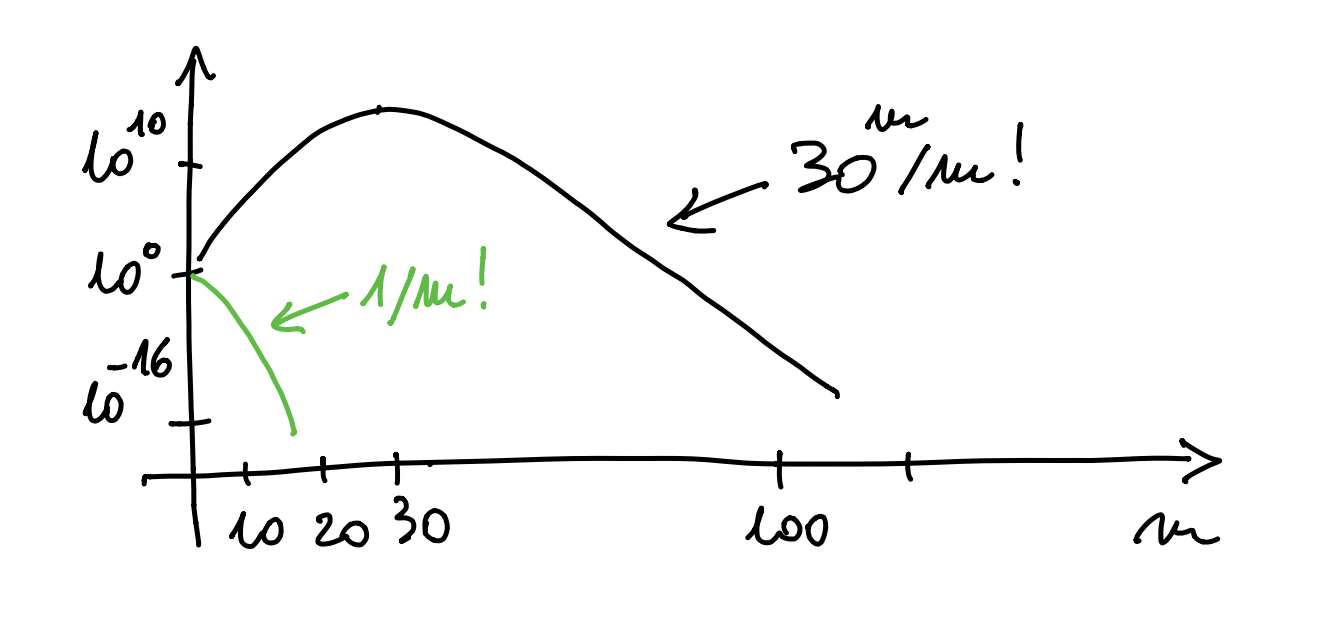
\includegraphics[width=0.5\textwidth]{grafo1.png}\par
\end{center}
Di conseguenza il calcolo di $e^x$ alla precisione di macchina con la formula di Taylor è molto efficiente per $x \leq 1$ ma richiede un polinomio di Taylor di grado $> \left[x\right]$ per $x>1$. D'altra parte sfruttando le proprietà della funzione esponenziale si può adottare il seguente trucco
\begin{equation*}
    e^x = (e^{\frac{x}{m}})^m
\end{equation*}
dove si scala la variabile $x$ con $m \in \mathbb{N} , m > x$ ad es. basta $m = [x]+1$, si approssima $e^y, y = \frac{x}{m}<1$, alla precisione di macchina con $t_{18}(y)$ e poi si calcola la potenza con l'algoritmo rapido basato sulla codifica binaria di m, a costo minore di $[2\cdot log_2(m)]$.\\
Si osservi anche che il calcolo di $t_{18} (y)$ è stabile, perché $(y>0)$ e tutte le operazioni coinvolte sono stabili (addizioni e moltiplicazioni con lo schema di Hörner, in tutto $(18\cdot 2=36$ flops). In definitiva con al massimo $36+2\left[ \log_2\left(\left[x\right]+1\right)\right]$ flops abbiamo un algoritmo che calcola \(e^x\) alla precisione di macchina (fino a \( x \approx{~} 708\) che è la soglia di overflow il costo è dell'ordine delle decine di flops).
Il Matlab adotta sostanzialmente questa tecnica per exp (con una formula più accurata di quella di Taylor per \(e^y\) con \(0<y\leq 1\) ).
\end{flushleft}
\end{document}
